\documentclass[12pt, a4paper]{book}

\usepackage[T1]{fontenc}
\usepackage[utf8]{inputenc}
\usepackage[charter, cal=cmcal]{mathdesign}
\usepackage[scaled=0.92]{helvet}
\usepackage{geometry}
\geometry{a4paper, top=30mm, bottom=30mm, inner=32mm, outer=25mm, marginparwidth=18mm}

\usepackage{amsmath, amsthm}
\usepackage[version=4]{mhchem}
\usepackage{graphicx}
\usepackage[dvipsnames,svgnames,table]{xcolor}
\usepackage{tikz}
\usetikzlibrary{arrows.meta, shapes.geometric, positioning, calc, backgrounds}
\usepackage{pgfplots}
\pgfplotsset{compat=1.18}
\usepackage{tcolorbox}
\tcbuselibrary{skins, breakable, theorems}
\usepackage{titlesec}
\usepackage{fancyhdr}
\usepackage{enumitem}
\usepackage{booktabs}
\usepackage{array}
\usepackage{multicol}
\usepackage{parskip}
\usepackage{siunitx}
\usepackage{colortbl}
\usepackage[colorlinks=true, linkcolor=BrickRed,
            urlcolor=NavyBlue, citecolor=ForestGreen]{hyperref}

\definecolor{JourneyColor}{HTML}{145A32}
\definecolor{ModuleColor}{HTML}{1E8449}
\definecolor{PuzzleColor}{HTML}{1A5276}
\definecolor{DiscoveryColor}{HTML}{B7950B}
\definecolor{WarningColor}{HTML}{C0392B}
\definecolor{ProblemColor}{HTML}{4A235A}
\definecolor{ReflectColor}{HTML}{117A65}
\definecolor{HistoryColor}{HTML}{6E2F1A}
\definecolor{DBlockColor}{HTML}{1B4F72}
\definecolor{SpinUp}{HTML}{1A5276}
\definecolor{SpinDown}{HTML}{922B21}

\newtcolorbox{puzzlebox}[1][]{enhanced,breakable,
  colback=PuzzleColor!6,colframe=PuzzleColor,fonttitle=\bfseries\sffamily,
  title={The Puzzle},attach boxed title to top left={yshift=-2mm,xshift=6mm},
  boxed title style={colback=PuzzleColor},borderline west={3pt}{0pt}{PuzzleColor},#1}

\newtcolorbox{discoverybox}[1][]{enhanced,breakable,
  colback=DiscoveryColor!8,colframe=DiscoveryColor,fonttitle=\bfseries\sffamily,
  title={Discovery},attach boxed title to top left={yshift=-2mm,xshift=6mm},
  boxed title style={colback=DiscoveryColor},borderline west={3pt}{0pt}{DiscoveryColor},#1}

\newtcolorbox{problembox}[1][]{enhanced,breakable,
  colback=ProblemColor!5,colframe=ProblemColor,fonttitle=\bfseries\sffamily,
  title={Problems},attach boxed title to top left={yshift=-2mm,xshift=6mm},
  boxed title style={colback=ProblemColor},borderline west={3pt}{0pt}{ProblemColor},#1}

\newtcolorbox{deepbox}[1][]{enhanced,breakable,
  colback=JourneyColor!5,colframe=JourneyColor,fonttitle=\bfseries\sffamily,
  title={Deep Problems},attach boxed title to top left={yshift=-2mm,xshift=6mm},
  boxed title style={colback=JourneyColor},borderline west={4pt}{0pt}{JourneyColor},#1}

\newtcolorbox{historybox}[1][]{enhanced,breakable,
  colback=HistoryColor!7,colframe=HistoryColor!60,fonttitle=\bfseries\sffamily\small,
  title={Historical Note},attach boxed title to top left={yshift=-2mm,xshift=6mm},
  boxed title style={colback=HistoryColor!80},#1}

\newtcolorbox{reflectionbox}[1][]{enhanced,breakable,
  colback=ReflectColor!6,colframe=ReflectColor,fonttitle=\bfseries\sffamily,
  title={Reflection},attach boxed title to top left={yshift=-2mm,xshift=6mm},
  boxed title style={colback=ReflectColor},borderline west={3pt}{0pt}{ReflectColor},#1}

\newtcolorbox{namedconcept}[2][]{enhanced,
  colback=ModuleColor!6,colframe=ModuleColor,fonttitle=\bfseries\sffamily\large,
  title={#2},attach boxed title to top left={yshift=-2mm,xshift=6mm},
  boxed title style={colback=ModuleColor},#1}

\titleformat{\chapter}[display]
  {\normalfont\sffamily\huge\bfseries\color{JourneyColor}}
  {\textcolor{JourneyColor!60}{\chaptertitlename\ \thechapter}}{10pt}{\Huge}
  [\vspace{2pt}\textcolor{JourneyColor}{\titlerule[1.5pt]}]
\titleformat{\section}
  {\normalfont\sffamily\Large\bfseries\color{ModuleColor}}
  {\thesection}{1em}{}[\textcolor{ModuleColor!40}{\titlerule[0.6pt]}]
\titleformat{\subsection}
  {\normalfont\sffamily\large\bfseries\color{JourneyColor!80}}{\thesubsection}{1em}{}
\titleformat{\subsubsection}
  {\normalfont\sffamily\normalsize\bfseries}{\thesubsubsection}{1em}{}

\pagestyle{fancy}
\fancyhf{}
\fancyhead[LE]{\small\sffamily\textcolor{JourneyColor}{\leftmark}}
\fancyhead[RO]{\small\sffamily\textcolor{ModuleColor}{\rightmark}}
\fancyfoot[C]{\small\thepage}
\renewcommand{\headrulewidth}{0.4pt}

\newcommand{\newterm}[1]{\textit{\textcolor{DiscoveryColor}{#1}}}
\newcommand{\important}[1]{\textcolor{ModuleColor}{\textbf{#1}}}

% Spin arrow helpers
\newcommand{\spinup}{\raisebox{0pt}{\tikz{\draw[-{Stealth[length=3pt]},thick,SpinUp](0,0)--(0,0.3);}}}
\newcommand{\spindown}{\raisebox{3pt}{\tikz{\draw[-{Stealth[length=3pt]},thick,SpinDown](0,0.3)--(0,0);}}}
\newcommand{\dbox}{\fbox{\phantom{XX}}}

\begin{document}
\setcounter{chapter}{2}
\chapter[Journey 3 --- The Periodic Table as a Discovery Engine]
        {Journey Three\\[8pt]
         \textcolor{ModuleColor}{\large The Periodic Table as a Discovery Engine}}
\setcounter{section}{3}

\section{Module 3.4 --- Transition Metals: The $d$-Block and Its Anomalies}
\label{sec:mod3.4}

\subsection*{Motivation}

The $s$- and $p$-block elements behave relatively simply:
their chemistry is dominated by one or two oxidation states,
and their periodic trends are smooth.

The $d$-block is different.
Ten elements span each transition series, all metals,
all with similar electronegativities and ionisation energies,
yet with strikingly different chemistry:
\begin{itemize}[nosep, leftmargin=2em]
  \item Multiple stable oxidation states
        (iron: +2 and +3; manganese: +2, +3, +4, +6, +7)
  \item Vivid colours (CuSO$_4$ is blue; \ce{K2Cr2O7} is orange;
        \ce{KMnO4} is deep purple)
  \item Magnetic properties (Fe, Co, Ni are ferromagnetic)
  \item Catalytic activity (Fe catalyses the Haber process;
        Pt catalyses \ce{H2}-\ce{O2} combination;
        Pd catalyses hydrogenation)
\end{itemize}

All of these arise from the partially filled $d$ subshell.
This module explains each property from its electron
configuration origin.

\subsection{The $d$-Block: Structure and Filling}

The first transition series runs from scandium ($Z=21$,
$[Ar]\,3d^1\,4s^2$) to zinc ($Z=30$, $[Ar]\,3d^{10}\,4s^2$).

\begin{center}
\small
\begin{tabular}{llllc}
\toprule
$Z$ & Element & Config & $d$-electrons & Unpaired $d$ \\
\midrule
21 & Sc & $[Ar]\,3d^1\,4s^2$ & 1 & 1 \\
22 & Ti & $[Ar]\,3d^2\,4s^2$ & 2 & 2 \\
23 & V  & $[Ar]\,3d^3\,4s^2$ & 3 & 3 \\
24 & \textbf{Cr} & $[Ar]\,3d^5\,4s^1$ & 5 & \textbf{5 (anomaly)} \\
25 & Mn & $[Ar]\,3d^5\,4s^2$ & 5 & 5 \\
26 & Fe & $[Ar]\,3d^6\,4s^2$ & 6 & 4 \\
27 & Co & $[Ar]\,3d^7\,4s^2$ & 7 & 3 \\
28 & Ni & $[Ar]\,3d^8\,4s^2$ & 8 & 2 \\
29 & \textbf{Cu} & $[Ar]\,3d^{10}\,4s^1$ & 10 & \textbf{0 (anomaly)} \\
30 & Zn & $[Ar]\,3d^{10}\,4s^2$ & 10 & 0 \\
\bottomrule
\end{tabular}
\end{center}

The two anomalies (Cr and Cu) arise from the extra stability
of half-filled ($d^5$) and fully-filled ($d^{10}$) subshells ---
the quantum mechanical version of Hund's rule extended.

\subsection{Multiple Oxidation States}

Unlike $s$- and $p$-block metals (which typically have
one stable oxidation state), transition metals exhibit
multiple oxidation states because the $3d$ and $4s$
electrons have similar energies and can both be removed.

\begin{center}
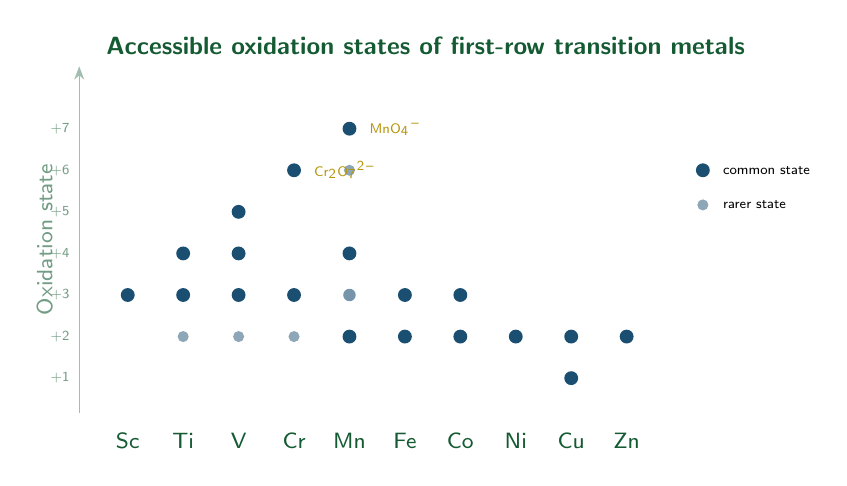
\begin{tikzpicture}[every node/.style={font=\sffamily\small}, scale=0.88]

  \node[font=\sffamily\small\bfseries, color=JourneyColor]
    at (5.5, 5.3) {Accessible oxidation states of first-row transition metals};

  % Y-axis: oxidation states
  \draw[-{Stealth}, thin, JourneyColor!40] (0.5,0) -- (0.5,5.0);
  \node[rotate=90, font=\sffamily\footnotesize, text=JourneyColor!60]
    at (0.0, 2.5) {Oxidation state};

  % X positions for each element
  % Sc=1.2, Ti=2.0, V=2.8, Cr=3.6, Mn=4.4, Fe=5.2, Co=6.0, Ni=6.8, Cu=7.6, Zn=8.4
  \foreach \xp/\elem in {
    1.2/Sc, 2.0/Ti, 2.8/V, 3.6/Cr,
    4.4/Mn, 5.2/Fe, 6.0/Co, 6.8/Ni, 7.6/Cu, 8.4/Zn
  }{
    \node[font=\sffamily\footnotesize, text=JourneyColor]
      at (\xp, -0.4) {\elem};
  }

  % Y-tick labels
  \foreach \y/\lbl in {0.5/+1, 1.1/+2, 1.7/+3, 2.3/+4, 2.9/+5, 3.5/+6, 4.1/+7} {
    \node[left, font=\sffamily\tiny, text=JourneyColor!60] at (0.5,\y) {\lbl};
  }

  % Draw dots for each accessible oxidation state
  % Common states as filled circles, rare as open
  % Format: x, y, filled?
  % Sc: +3
  \fill[DBlockColor] (1.2,1.7) circle (0.10cm);
  % Ti: +2,+3,+4
  \fill[DBlockColor!50] (2.0,1.1) circle (0.08cm);
  \fill[DBlockColor]    (2.0,1.7) circle (0.10cm);
  \fill[DBlockColor]    (2.0,2.3) circle (0.10cm);
  % V: +2,+3,+4,+5
  \fill[DBlockColor!50] (2.8,1.1) circle (0.08cm);
  \fill[DBlockColor]    (2.8,1.7) circle (0.10cm);
  \fill[DBlockColor]    (2.8,2.3) circle (0.10cm);
  \fill[DBlockColor]    (2.8,2.9) circle (0.10cm);
  % Cr: +2,+3,+6
  \fill[DBlockColor!50] (3.6,1.1) circle (0.08cm);
  \fill[DBlockColor]    (3.6,1.7) circle (0.10cm);
  \fill[DBlockColor]    (3.6,3.5) circle (0.10cm);
  % Mn: +2,+3,+4,+6,+7
  \fill[DBlockColor]    (4.4,1.1) circle (0.10cm);
  \fill[DBlockColor!60] (4.4,1.7) circle (0.09cm);
  \fill[DBlockColor]    (4.4,2.3) circle (0.10cm);
  \fill[DBlockColor!50] (4.4,3.5) circle (0.08cm);
  \fill[DBlockColor]    (4.4,4.1) circle (0.10cm);
  % Fe: +2,+3
  \fill[DBlockColor]    (5.2,1.1) circle (0.10cm);
  \fill[DBlockColor]    (5.2,1.7) circle (0.10cm);
  % Co: +2,+3
  \fill[DBlockColor]    (6.0,1.1) circle (0.10cm);
  \fill[DBlockColor]    (6.0,1.7) circle (0.10cm);
  % Ni: +2
  \fill[DBlockColor]    (6.8,1.1) circle (0.10cm);
  % Cu: +1,+2
  \fill[DBlockColor]    (7.6,0.5) circle (0.10cm);
  \fill[DBlockColor]    (7.6,1.1) circle (0.10cm);
  % Zn: +2
  \fill[DBlockColor]    (8.4,1.1) circle (0.10cm);

  % Legend
  \fill[DBlockColor]    (9.5,3.5) circle (0.10cm);
  \node[right, font=\sffamily\tiny] at (9.65,3.5) {common state};
  \fill[DBlockColor!50] (9.5,3.0) circle (0.08cm);
  \node[right, font=\sffamily\tiny] at (9.65,3.0) {rarer state};

  % Mn=7 annotation
  \node[font=\sffamily\tiny, text=DiscoveryColor, right]
    at (4.55,4.1) {\ce{MnO4-}};
  % Cr=6 annotation
  \node[font=\sffamily\tiny, text=DiscoveryColor, right]
    at (3.75,3.5) {\ce{Cr2O7^{2-}}};

\end{tikzpicture}
\end{center}

\vspace{0.4em}

The pattern is clear: maximum oxidation state peaks at
manganese (+7) at the centre of the series,
then decreases toward zinc.
This mirrors the number of $d$ electrons available for bonding.

\subsection{Colour in Transition Metal Compounds}

\begin{puzzlebox}
Consider these observations:

\begin{center}
\small
\begin{tabular}{llll}
\toprule
Compound & Colour & Ion & $d$-electrons \\
\midrule
\ce{CuSO4} solution & blue     & \ce{Cu^{2+}} & $d^9$ \\
\ce{CuCl}  solution & colourless & \ce{Cu+}  & $d^{10}$ \\
\ce{FeCl3} solution & yellow-brown & \ce{Fe^{3+}} & $d^5$ \\
\ce{FeCl2} solution & pale green & \ce{Fe^{2+}} & $d^6$ \\
\ce{KMnO4} solution & deep purple & \ce{Mn^{7+}} & $d^0$ \\
\ce{ZnSO4} solution & colourless & \ce{Zn^{2+}} & $d^{10}$ \\
\bottomrule
\end{tabular}
\end{center}

\begin{enumerate}[label=(\alph*), leftmargin=*]
  \item \ce{Cu+} (d$^{10}$, full) and \ce{Zn^{2+}} (d$^{10}$, full)
        are both colourless.
        \ce{Mn^{7+}} (d$^0$, empty) is also colourless.
        What pattern do you notice?
        Form a hypothesis: what is necessary for colour?

  \item \ce{Cu^{2+}} (d$^9$) is blue.
        This means it absorbs red-orange light ($\sim$650--700 nm)
        and transmits blue.
        What energy in eV corresponds to 650 nm light?

  \item The same \ce{Cu^{2+}} ion appears different colours
        in different solvents:
        deep blue in water, green in hydrochloric acid
        (where Cl$^-$ replaces water as a ligand).
        What does this tell you about what causes
        the energy gap that absorbs light?
\end{enumerate}
\end{puzzlebox}

The answer lies in \newterm{crystal field theory}.
When ligands (molecules or ions surrounding the metal)
approach a transition metal ion, they interact with
the $d$ orbitals differently depending on their geometry.

In an octahedral complex (6 ligands), the five $d$ orbitals
split into two groups:
\begin{itemize}[nosep, leftmargin=2em]
  \item $e_g$ orbitals (point at ligands): raised in energy
  \item $t_{2g}$ orbitals (point between ligands): lower in energy
\end{itemize}

The energy gap $\Delta_o$ (the octahedral crystal field splitting)
depends on the metal, oxidation state, and ligands.
Transitions between $t_{2g}$ and $e_g$ absorb visible light.

\begin{center}
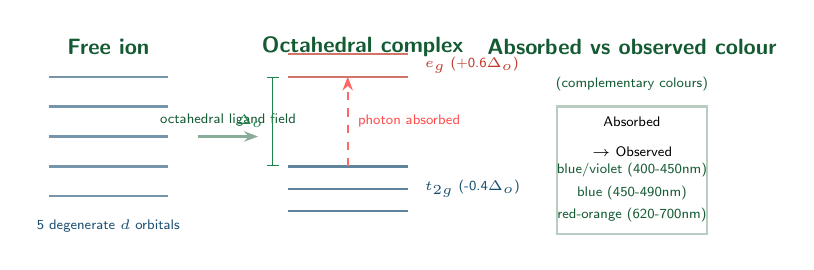
\begin{tikzpicture}[every node/.style={font=\sffamily\small}, scale=0.95]

  % Free ion (5 degenerate d orbitals)
  \begin{scope}[xshift=0cm]
    \node[font=\sffamily\footnotesize\bfseries, color=JourneyColor]
      at (1.0, 3.0) {Free ion};
    \foreach \y in {1.0, 1.4, 1.8, 2.2, 2.6} {
      \draw[thick, DBlockColor!60] (0.2,\y) -- (1.8,\y);
    }
    \node[font=\sffamily\tiny, text=DBlockColor]
      at (1.0, 0.6) {5 degenerate $d$ orbitals};
  \end{scope}

  % Arrow
  \draw[-{Stealth[length=5pt]}, thick, JourneyColor!50]
    (2.2, 1.8) -- (3.0, 1.8)
    node[midway, above, font=\sffamily\tiny, text=JourneyColor]
      {octahedral ligand field};

  % Octahedral splitting
  \begin{scope}[xshift=3.2cm]
    \node[font=\sffamily\footnotesize\bfseries, color=JourneyColor]
      at (1.2, 3.0) {Octahedral complex};
    % e_g (2 orbitals, raised)
    \draw[thick, WarningColor!70] (0.2,2.6) -- (1.8,2.6);
    \draw[thick, WarningColor!70] (0.2,2.9) -- (1.8,2.9);
    \node[right, font=\sffamily\tiny, text=WarningColor]
      at (1.9,2.75) {$e_g$ (+0.6$\Delta_o$)};
    % t_2g (3 orbitals, lowered)
    \draw[thick, DBlockColor!70] (0.2,0.8) -- (1.8,0.8);
    \draw[thick, DBlockColor!70] (0.2,1.1) -- (1.8,1.1);
    \draw[thick, DBlockColor!70] (0.2,1.4) -- (1.8,1.4);
    \node[right, font=\sffamily\tiny, text=DBlockColor]
      at (1.9,1.1) {$t_{2g}$ (-0.4$\Delta_o$)};
    % Delta_o bracket
    \draw[{|}-{|}, thin, ModuleColor]
      (0.0, 1.4) -- (0.0, 2.6)
      node[midway, left, font=\sffamily\tiny, text=ModuleColor]
        {$\Delta_o$};
    % Photon absorption arrow
    \draw[-{Stealth[length=5pt]}, thick, red!60, dashed]
      (1.0,1.4) -- (1.0,2.6)
      node[midway, right, font=\sffamily\tiny, text=red!70]
        {photon absorbed};
  \end{scope}

  % Colour wheel annotation
  \begin{scope}[xshift=6.8cm, yshift=0.5cm]
    \node[font=\sffamily\footnotesize\bfseries, color=JourneyColor]
      at (1.2, 2.5) {Absorbed vs observed colour};
    \node[font=\sffamily\tiny, color=JourneyColor] at (1.2,2.0)
      {(complementary colours)};
    \draw[thick, JourneyColor!30] (0.2,0) rectangle (2.2,1.7);
    \node[font=\sffamily\tiny] at (1.2,1.5) {Absorbed};
    \node[font=\sffamily\tiny] at (1.2,1.1) {$\to$ Observed};
    \foreach \lbl/\abs/\obs/\yp in {
      {blue/violet (400-450nm)}/{yellow-orange}/yellow/0.85,
      {blue (450-490nm)}/{orange}/orange/0.55,
      {red-orange (620-700nm)}/{blue}/blue/0.25
    }{
      \node[font=\sffamily\tiny, text=JourneyColor] at (1.2,\yp) {\lbl};
    }
  \end{scope}

\end{tikzpicture}
\end{center}

The \newterm{spectrochemical series} orders ligands by their
ability to split the $d$ levels ($\Delta_o$):
\[
  \text{I}^- < \text{Br}^- < \text{Cl}^- < \text{F}^- <
  \text{OH}^- < \text{H}_2\text{O} < \text{NH}_3 <
  \text{en} < \text{CN}^- < \text{CO}
\]

``Weak field'' ligands (I$^-$, Cl$^-$) give small $\Delta_o$
and absorb lower-energy (red) light.
``Strong field'' ligands (CN$^-$, CO) give large $\Delta_o$
and absorb higher-energy (blue-violet) light.

\subsection{Magnetism: Unpaired Electrons and Spin}

Transition metal compounds are magnetic because of
\emph{unpaired electrons}.

\begin{namedconcept}{Paramagnetism and Ferromagnetism}
\textbf{Paramagnetism}: an atom or ion with unpaired
electrons is weakly attracted into a magnetic field.
The magnetic moment $\mu$ (in Bohr magnetons) is:
\[
  \mu = \sqrt{n(n+2)}\,\mu_B
\]
where $n$ is the number of unpaired electrons.

\textbf{Ferromagnetism}: in Fe, Co, and Ni, the unpaired
electrons of neighbouring atoms align spontaneously
over large domains, giving strong permanent magnetism.
This requires both unpaired electrons \emph{and}
the right crystal structure for long-range ordering.
\end{namedconcept}

\vspace{0.5em}

The number of unpaired electrons depends on both the
electron configuration and the crystal field splitting.

For a $d^6$ metal (e.g.\ \ce{Fe^{2+}}):
\begin{itemize}[nosep, leftmargin=2em]
  \item \textbf{Weak field} (small $\Delta_o$): electrons
        spread across all five $d$ orbitals (Hund's rule wins)
        --- \newterm{high spin}, 4 unpaired electrons.
  \item \textbf{Strong field} (large $\Delta_o$): electrons
        pair up in the lower $t_{2g}$ orbitals first
        --- \newterm{low spin}, 0 unpaired electrons.
\end{itemize}

\begin{center}
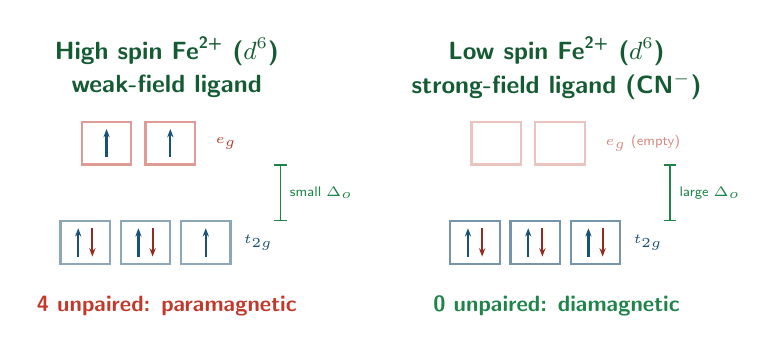
\begin{tikzpicture}[every node/.style={font=\sffamily\small}, scale=0.9]

  % High spin Fe2+ (d6, weak field)
  \begin{scope}[xshift=0cm]
    \node[font=\sffamily\small\bfseries, color=JourneyColor]
      at (1.5, 3.5) {High spin \ce{Fe^{2+}} ($d^6$)};
    \node[font=\sffamily\small\bfseries, color=JourneyColor]
      at (1.5, 3.0) {weak-field ligand};
    % e_g (2 boxes, each with 1 up)
    \foreach \x in {0.3, 1.2} {
      \draw[thick, WarningColor!50] (\x,1.9) rectangle (\x+0.7,2.5);
      \draw[-{Stealth[length=3pt]}, thick, SpinUp]
        (\x+0.35,2.0) -- (\x+0.35,2.4);
    }
    \node[right, font=\sffamily\tiny, text=WarningColor]
      at (2.05,2.2) {$e_g$};
    % t_2g (3 boxes: 2 paired, 1 single)
    \foreach \x in {0.0, 0.85} {
      \draw[thick, DBlockColor!50] (\x,0.5) rectangle (\x+0.7,1.1);
      \draw[-{Stealth[length=3pt]}, thick, SpinUp]
        (\x+0.25,0.6) -- (\x+0.25,1.0);
      \draw[-{Stealth[length=3pt]}, thick, SpinDown]
        (\x+0.45,1.0) -- (\x+0.45,0.6);
    }
    \draw[thick, DBlockColor!50] (1.7,0.5) rectangle (2.4,1.1);
    \draw[-{Stealth[length=3pt]}, thick, SpinUp]
      (2.05,0.6) -- (2.05,1.0);
    \node[right, font=\sffamily\tiny, text=DBlockColor]
      at (2.45,0.8) {$t_{2g}$};
    \node[font=\sffamily\footnotesize\bfseries, text=WarningColor]
      at (1.5,-0.1) {4 unpaired: paramagnetic};
  \end{scope}

  % Low spin Fe2+ (d6, strong field)
  \begin{scope}[xshift=5.5cm]
    \node[font=\sffamily\small\bfseries, color=JourneyColor]
      at (1.5, 3.5) {Low spin \ce{Fe^{2+}} ($d^6$)};
    \node[font=\sffamily\small\bfseries, color=JourneyColor]
      at (1.5, 3.0) {strong-field ligand (CN$^-$)};
    % e_g empty
    \foreach \x in {0.3, 1.2} {
      \draw[thick, WarningColor!30] (\x,1.9) rectangle (\x+0.7,2.5);
    }
    \node[right, font=\sffamily\tiny, text=WarningColor!60]
      at (2.05,2.2) {$e_g$ (empty)};
    % t_2g fully paired
    \foreach \x in {0.0, 0.85, 1.7} {
      \draw[thick, DBlockColor!60] (\x,0.5) rectangle (\x+0.7,1.1);
      \draw[-{Stealth[length=3pt]}, thick, SpinUp]
        (\x+0.25,0.6) -- (\x+0.25,1.0);
      \draw[-{Stealth[length=3pt]}, thick, SpinDown]
        (\x+0.45,1.0) -- (\x+0.45,0.6);
    }
    \node[right, font=\sffamily\tiny, text=DBlockColor]
      at (2.45,0.8) {$t_{2g}$};
    \node[font=\sffamily\footnotesize\bfseries, text=ModuleColor]
      at (1.5,-0.1) {0 unpaired: diamagnetic};
  \end{scope}

  % Delta_o labels
  \draw[{|}-{|}, thin, ModuleColor] (3.1,1.1) -- (3.1,1.9)
    node[right, midway, font=\sffamily\tiny, text=ModuleColor]
      {small $\Delta_o$};
  \draw[{|}-{|}, thin, ModuleColor] (8.6,1.1) -- (8.6,1.9)
    node[right, midway, font=\sffamily\tiny, text=ModuleColor]
      {large $\Delta_o$};

\end{tikzpicture}
\end{center}

This has real biological consequences.
Haemoglobin contains an Fe$^{2+}$ ion.
When \ce{O2} binds, it becomes a strong-field ligand
and forces the iron into low-spin, diamagnetic state.
When \ce{CO} binds (carbon monoxide poisoning), the complex
is also low-spin but cannot release the CO --- the Fe
is permanently blocked from carrying oxygen.

\subsection{Catalysis: Why Transition Metals Catalyse}

Transition metals are the world's most important catalysts
because of two properties that arise from the $d$-block:

\begin{enumerate}[nosep, leftmargin=2em]
  \item \textbf{Variable oxidation state}: the metal can
        accept and donate electrons, mediating redox reactions.
  \item \textbf{Ability to adsorb reactants}: $d$ orbitals
        can form weak, reversible bonds with molecules
        (like H$_2$, N$_2$, CO), holding them in the
        right geometry for reaction without permanently
        consuming the catalyst.
\end{enumerate}

\begin{center}
\small
\begin{tabular}{llll}
\toprule
Catalyst & Reaction & Why it works \\
\midrule
Fe & \ce{N2 + 3H2 -> 2NH3} (Haber) & Dissociates N$_2$ on surface \\
Pt/Pd & Hydrogenation \ce{C=C -> C-C} & Adsorbs H$_2$, weakens H-H bond \\
V$_2$O$_5$ & \ce{SO2 -> SO3} (Contact process) & V$^{5+}$ $\to$ V$^{4+}$ $\to$ V$^{5+}$ cycle \\
Mn$^{2+}$ & \ce{H2O2 -> H2O + O2} & Variable oxidation state \\
Ni & Steam reforming of hydrocarbons & C-H bond activation on surface \\
\bottomrule
\end{tabular}
\end{center}

\begin{problembox}
\begin{enumerate}[label=\textbf{\arabic*.}]
  \item \textbf{Crystal field and colour.}
        \begin{enumerate}[label=(\alph*)]
          \item \ce{[Ti(H2O)6]^{3+}} absorbs light at 493 nm
                (blue-green). What colour does this complex appear?
          \item Calculate the crystal field splitting energy
                $\Delta_o$ in kJ/mol for this complex.
          \item \ce{[Ti(CN)6]^{3-}} has a larger $\Delta_o$
                than the water complex.
                Will it absorb at longer or shorter wavelength?
                Predict the colour.
          \item Ti$^{3+}$ has electron configuration $d^1$.
                Draw the $t_{2g}$/$e_g$ energy level diagram
                showing where the electron sits before and
                after absorbing a photon.
        \end{enumerate}

  \item \textbf{Magnetic moments.}
        Calculate the expected magnetic moment $\mu = \sqrt{n(n+2)}\,\mu_B$
        for the following high-spin complexes:
        \begin{enumerate}[label=(\alph*)]
          \item \ce{[Mn(H2O)6]^{2+}} ($d^5$, 5 unpaired)
          \item \ce{[Fe(H2O)6]^{3+}} ($d^5$, 5 unpaired)
          \item \ce{[Co(H2O)6]^{2+}} ($d^7$, 3 unpaired)
          \item \ce{[Ni(H2O)6]^{2+}} ($d^8$, 2 unpaired)
          \item \ce{[Zn(H2O)6]^{2+}} ($d^{10}$, 0 unpaired)
        \end{enumerate}
        Which is most strongly paramagnetic?
        Which is diamagnetic?

  \item \textbf{Catalytic cycles.}
        The industrial Contact process converts SO$_2$ to SO$_3$
        using \ce{V2O5} catalyst:
        \begin{align*}
          \text{Step 1:} & \quad
            \ce{SO2 + V2O5 -> SO3 + V2O4} \\
          \text{Step 2:} & \quad
            \ce{V2O4 + \tfrac{1}{2}O2 -> V2O5}
        \end{align*}
        \begin{enumerate}[label=(\alph*)]
          \item What is the oxidation state of vanadium in
                \ce{V2O5} and in \ce{V2O4}?
          \item Show that the overall reaction (sum of
                both steps) is \ce{SO2 + \frac{1}{2}O2 -> SO3}.
          \item Why is the catalyst not consumed?
          \item Why would a main-group element (like Na or Ca)
                be unable to serve as a catalyst for this
                reaction?
        \end{enumerate}
\end{enumerate}
\end{problembox}

\subsection*{Deep Problems}

\begin{deepbox}
\begin{enumerate}[label=\textbf{D\arabic*.}]

  \item \textbf{Haemoglobin and the Iron Centre.}

        The active site of haemoglobin is a haem group ---
        an Fe$^{2+}$ ion coordinated in a square planar
        arrangement by four nitrogen atoms of a porphyrin ring,
        with a histidine residue below and a binding site above.

        \begin{enumerate}[label=(\alph*)]
          \item In deoxyhaemoglobin (no O$_2$ bound),
                Fe$^{2+}$ is high-spin ($d^6$, 4 unpaired).
                When O$_2$ binds, it becomes low-spin
                (0 unpaired electrons).
                Blood is actually paramagnetic when deoxygenated
                and diamagnetic when oxygenated.
                This difference can be detected by MRI.
                Explain the basis of BOLD fMRI imaging
                (blood oxygenation level-dependent signal),
                which maps brain activity.
          \item The Fe$^{2+}$ ion in deoxyhaemoglobin sits
                slightly above the plane of the porphyrin ring
                (because the high-spin state makes the ion
                slightly larger).
                When O$_2$ binds, it becomes low-spin,
                the ion contracts, and pulls into the plane.
                This movement is transmitted to the rest
                of the protein, triggering a conformational
                change that makes the other three haem groups
                in haemoglobin bind O$_2$ more readily
                (\newterm{cooperativity}).
                Describe cooperativity in your own words.
                Why is it biologically essential for
                efficient oxygen delivery?
          \item Carbon monoxide (\ce{CO}) is a stronger-field
                ligand than O$_2$ and binds Fe$^{2+}$ about
                250 times more tightly.
                Explain, using the crystal field model,
                why CO is such a potent poison.
        \end{enumerate}

  \item \textbf{The Irving-Williams Series.}

        The stability constants of complexes with divalent
        first-row transition metal ions follow the order:
        \[
          \text{Mn}^{2+} < \text{Fe}^{2+} < \text{Co}^{2+} <
          \text{Ni}^{2+} < \text{Cu}^{2+} > \text{Zn}^{2+}
        \]
        (Cu$^{2+}$ forms the most stable complexes.)

        \begin{enumerate}[label=(\alph*)]
          \item The general trend (Mn to Cu increasing) reflects
                increasing $Z_\text{eff}$ across the series.
                Explain why increasing $Z_\text{eff}$ makes
                the metal a better Lewis acid and therefore
                forms more stable complexes.
          \item The drop from Cu to Zn is caused by the
                $d^{10}$ configuration of Zn$^{2+}$.
                A full $d$ shell has no crystal field
                stabilisation energy (CFSE).
                Explain what CFSE is and why its absence
                weakens Zn$^{2+}$ complexes.
          \item Cu$^{2+}$ complexes often distort from perfect
                octahedral geometry --- four short bonds
                and two long bonds along one axis
                (\newterm{Jahn-Teller distortion}).
                This arises because the $d^9$ configuration
                puts one electron in the $e_g$ level
                asymmetrically.
                Sketch the orbital diagram showing this
                asymmetry and explain why it lowers energy.
        \end{enumerate}

\end{enumerate}
\end{deepbox}

\subsection*{Reflection}

\begin{reflectionbox}
\begin{enumerate}[label=\textbf{R\arabic*.}]
  \item The colour of copper sulphate solution, the magnetism
        of iron, the toxicity of carbon monoxide, and the
        efficiency of industrial catalysts all trace back to
        the energy splitting of five $d$ orbitals by six
        surrounding ligands.
        \textbf{Is it surprising that such macroscopic,
        practical phenomena reduce to a quantum mechanical
        energy level diagram?}
        What does this tell us about the relationship
        between chemistry and physics?

  \item Transition metal catalysts underpin the Haber process
        (feeding $\sim$3 billion people), hydrogenation
        (food industry), and catalytic converters (reducing
        air pollution).
        \textbf{Would these technologies have been possible
        without the periodic table as a guide?}
        How does the table function as a map for
        practical materials discovery?

  \item BOLD fMRI detects the magnetic difference between
        oxygenated and deoxygenated blood to image brain
        activity.
        \textbf{Trace the chain of reasoning from the
        Schr\"{o}dinger equation in 1926 to a 21st-century
        neuroscience tool.}
        How many ``layers'' of scientific development
        separate the fundamental theory from the application?
\end{enumerate}
\end{reflectionbox}

\vspace{1.5em}
\begin{center}
\begin{tcolorbox}[enhanced, colback=DiscoveryColor!8, colframe=DiscoveryColor,
  width=0.88\textwidth, arc=3pt]
\centering\sffamily\small
\textbf{What we invented in this module.}\\[4pt]
The $d$-block is where the periodic table becomes biochemistry,
materials science, and industrial chemistry simultaneously.
Multiple oxidation states arise from the near-degenerate $3d$
and $4s$ levels.
Colour arises from crystal field splitting of $d$ orbitals
by surrounding ligands.
Magnetism arises from unpaired electrons, with the magnetic
state controllable by ligand choice.
Catalytic activity arises from the unique ability of partially
filled $d$ orbitals to bind, activate, and release molecules
reversibly.
All of this is a direct consequence of where these elements
sit in the periodic table --- in the block where the $d$
subshell is being filled.
\end{tcolorbox}
\end{center}

\vspace{2em}
\noindent\textcolor{JourneyColor!40}{\rule{\textwidth}{0.6pt}}
\begin{center}
\textit{\sffamily\small
Module 3.4 complete. Continue to Module 3.5:\\
\textbf{Journey 3 Synthesis: The Table as a Prediction Engine}.}
\end{center}

\end{document}